% !TEX ROOT = ../ersti.tex
\section{Überblick}
\label{hopo}



Es ist zwar sehr einleuchtend, dass sich die Hochschulpolitik mit den Belangen der Hochschulteilnehmerinnen beschäftigt, jedoch sind die Grenzen der Hochschulpolitik nicht eindeutig. Denn wie so häufig in der Politik, hängt alles miteinander zusammen: Der lokale ÖPNV und das Semesterticket, der teure Wohnungsmarkt und die Studierendenwohnheime sowie befristete Arbeitsstellen und Tutorien. Indirekt -- aber manchmal auch ziemlich direkt –- sind Studentinnen von politischen Entscheidungen betroffen. Im Folgenden werden die verschiedenen Ebenen und deren Gremien vorgestellt, in denen Studentinnen bei Entscheidungsprozessen mehr oder weniger mitmischen können. Die Gremien lassen sich grob in studentische Selbstverwaltung einerseits sowie akademische Selbstverwaltung andererseits trennen.


\subsection{Studienkommission}
Für jedes Fach gibt es eine Studien\-kom\-mis\-sion, welche sich um die Themen Studium und Lehre ihrer Studiengänge kümmert. Die besprochenen Themen betreffen uns Studentinnen direkt, da es um Studiengangsgestaltung und Lehrqualität geht. Neben der Studiendekanin sind Professorinnen, Mittelbaulerinnen (z.B. wissenschaftliche Mitarbeiterinnen und Privatdozentinnen) und vier -- also verhältnismäßig viele -- Studentinnen Mitglieder des Gremiums, weshalb dieses Gremium aus Sicht der Studentinnen am besten geeignet ist, um die studentische Meinung zu vertreten.

Jede Änderung von Prüfungsordnungen, Modulhandbüchern und Studienplänen sowie das Lehrprogramm jedes Semesters wird in den Studienkommissionen besprochen und abgestimmt. Außerdem wird die Qualität der Lehre anhand von Ergebnissen der Lehrveranstaltungsevaluationen und Studiengangsbefragungen analysiert und anschließend versucht, zu verbessern. Die Entscheidungen betreffen einen als Studentin direkt im Studienalltag. Die studentischen Vertreterinnen werden von der Fachschaft vorgeschlagen und dann vom jeweiligen Fakultätsrat bestätigt.

\begin{figure}[b]
    \centering
    \includegraphics[width=.9\linewidth]{bilder/duty_calls.png}
\end{figure}

\vspace{-3mm}

\subsection{Fakultätsrat}

\begin{figure*}[b]
    \centering
    \begin{subfigure}{.3\textwidth}
        \includegraphics[height=3cm]{bilder/dear_CERN_1.png}
        \vspace{7mm}
    \end{subfigure}
    \begin{subfigure}{.3\textwidth}
        \includegraphics[height=3cm]{bilder/dear_CERN_2.png}
        \vspace{7mm}
    \end{subfigure}
    \begin{subfigure}{.3\textwidth}
        \includegraphics[height=3cm]{bilder/dear_CERN_3.png}
        \vspace{7mm}
    \end{subfigure}
    \begin{subfigure}{.3\textwidth}
        \includegraphics[height=3cm]{bilder/dear_CERN_4.png}
    \end{subfigure}
    \begin{subfigure}{.3\textwidth}
        \includegraphics[height=3cm]{bilder/dear_CERN_5.png}
    \end{subfigure}
    \begin{subfigure}{.3\textwidth}
        \includegraphics[height=3cm]{bilder/dear_CERN_6.png}
    \end{subfigure}
\end{figure*}

Jede Fakultät besitzt als zentrales Gremium einen Fakultätsrat, der ebenso wie die Studienkommission während der Vorlesungszeit in der Regel monatlich tagt. Anders als in den Studienkommissionen, welche den Fakultätsräten untergeordnet sind, besitzen die Professorinnen in den Fakultätsräten eine eindeutige Mehrheit gegenüber den Mittelbaulerinnen und studentischen Vertreterinnen. Letztere kann man einmal im Jahr per Wahl bestimmen, wobei die Fachschaft häufig die einzige Liste mit Kandidatinnen aufstellt.

Im Fakultätsrat werden alle Angelegenheiten der Fakultät besprochen, insbesondere Berufungen von neuen Professorinnen, Forschungsfreisemester sowie andere wegweisende Entscheidungen. Die Ergebnisse der Studienkommission müssen in der Regel im Fakultätsrat bestätigt werden, jedoch werden diese häufig einfach durchgewunken, da sich der Fakultätsrat mit deutlich mehr als nur Studium und Lehre beschäftigt. Im Fakultätsrat werden also auch schon viele Themen diskutiert, die Studentinnen nur sehr indirekt betreffen.

Angeführt wird eine Fakultät durch eine Dekanin, sowie den Studiendekaninnen und Prodekaninnen als Fakultätsvorstand. Unsere Studiengänge gehören zu den Fakultäten für Physik und Astronomie sowie Mathematik und Informatik, wobei \dekanphysik\ in der ersteren und \dekanmathe\ in der letzteren Dekan ist. Die 12 Fakultäten der Universität Heidelberg sind weiter aufgegliedert in Institute und Seminare, welche wiederum in fachspezifischere Arbeitsgruppen unterteilt sind.

\subsection{Senat und universitätsweite Gremien}
Da sich auch die verschiedenen Fakultäten untereinander absprechen müssen, gibt es zentrale universitätsweite Gremien, wobei die Struktur ähnlich wie auf Fakultätsebene ist. Die Professorinnen haben eine deutliche Mehrheit, denn neben den 16 gewählten Professorinnen und nur 4 Studentinnen sind auch noch der Rektor, die vier Prorektorinnen, der Kanzler sowie alle 12 Dekaninnen Senatsmitglieder. Hier herrscht also kaum studentische Mitgestaltungsmöglichkeit. Jedoch hat der Senat diverse Unterausschüsse, insbesondere den Senatsausschuss für Lehre (SAL), welcher sich ähnlich wie die Studienkommissionen alleine mit den Themen Studium und Lehre befasst, diesmal nur mit Themen, die alle Fakultäten betreffen. Zum Beispiel wurde lange über Anwesenheitspflicht und den Master of Ed\-u\-ca\-tion gesprochen, sodass nicht jede Fakultät eine eigene Regelung treffen muss. Neben dem Bestätigen und Durchwinken von Entscheidungen der Fakultäten, beschäftigt sich der Senat hauptsächlich mit strategischen und richtungsweisenden Entscheidungen der Universität.
Diese betreffen hauptsächlich professorale Angelegenheiten der Forschung und eher weniger, aber umso wichtigere studentische Belange.

Der Rektor der Universität ist zurzeit Bernhard Eitel. Als Leiter des Rektorats stellt er mit diesem die Hochschulleitung dar und vertritt die Hochschule nach innen und außen, wie es so schön heißt. Die vier Prorektorinnen sind jeweils für bestimmte Bereiche zuständig, unter anderem gibt es den Bereich Studium und Lehre.

Die organisatorischen Aufgaben der Universität werden von der (Zentralen) Universitätsverwaltung (ZUV) übernommen, welche von dem Kanzler \kanzler\ geleitet wird und in acht Dezernate gegliedert ist. Die ZUV sitzt größtenteils im Carolinum in der Seminarstraße~2 und ist für Studentinnen eine wichtige Anlaufstelle zum Beispiel für die Immatrikulation, die zentrale Studienberatung, das Deutschlandstipendium und Wahlen für Universitätsgremien.

% \begin{figure*}[b]
%     \centering
%     \begin{subfigure}{.3\textwidth}
%         \includegraphics[height=3cm]{bilder/inequivalence_principle_1.png}
%         \vspace{7mm}
%     \end{subfigure}
%     \begin{subfigure}{.3\textwidth}
%         \includegraphics[height=3cm]{bilder/inequivalence_principle_2.png}
%         \vspace{7mm}
%     \end{subfigure}
%     \begin{subfigure}{.3\textwidth}
%         \includegraphics[height=3cm]{bilder/inequivalence_principle_3.png}
%         \vspace{7mm}
%     \end{subfigure}
%     \begin{subfigure}{.3\textwidth}
%         \includegraphics[height=3cm]{bilder/inequivalence_principle_4.png}
%     \end{subfigure}
%     \begin{subfigure}{.3\textwidth}
%         \includegraphics[height=3cm]{bilder/inequivalence_principle_5.png}
%     \end{subfigure}
%     \begin{subfigure}{.3\textwidth}
%         \includegraphics[height=3cm]{bilder/inequivalence_principle_6.png}
%     \end{subfigure}
% \end{figure*}
Ein interessantes Gremium, das jedoch kaum eine Studentin kennt, ist der Universitätsrat, welcher eine Art Aufsichtsrat für die Universität, insbesondere das Rektorat darstellt. Sechs der elf Mitglieder sind externe Personen aus der Wirtschaft, Politik und Gesellschaft, die anderen fünf interne Mitglieder, davon eine studentische Vertreterin. Alle werden vom Wissenschaftsministerium auf Vorschlag einer Findungskommission benannt.Der Universitätsrat hat das letzte Wort in Finanzangelegenheiten und somit wesentlichen Einfluss auf die künftige Entwicklung der Universität, jedoch keinen direkten Bezug zum studentischen Alltag.



Das Studierendenwerk ist übrigens nicht Teil der Universität, sondern eine eigenständige Anstalt öffentlichen Rechts, die aber sehr stark mit der Universität zusammenarbeitet.

\subsection{Fachschaft}
Neben diesen Gremien der akademischen Selbstverwaltung gibt es auch eine ähnliche Struktur in der studentischen Selbstverwaltung. Jedes Fach besitzt eine Studienfachschaft -- bei uns Mathematik, Informatik und Physik -- welche aus allen Studentinnen besteht, die dieses Fach studieren. Da sich bei unseren Fächern viele Module überschneiden, ergibt es Sinn, dass wir als gemeinsame Fachschaft zusammenarbeiten und nicht nach Fächern getrennt. Nur so lassen sich zum Beispiel große Projekte wie der Vorkurs oder die MathPhysTheo organisieren. Aber wenn es um formale Angelegenheiten wie zum Beispiel Wahlen oder den Fachschaftsrat geht, dann werden wir in Studienfachschaften aufgeteilt.

Die Fachschaft besteht im groben aus zwei Organen, der Fachschaftsvollversammlung -- welche wir traditionell als Fachschaftssitzung bezeichnen -- und dem Fachschaftsrat, der bei uns jedoch nur die Entscheidungen der Fachschaftssitzung ausführt. Die drei Fachschaftsräte der jeweiligen Studienfachschaft können einmal im Jahr gewählt werden, in die Fachschaftssitzungen kann jeder kommen und hat automatisch Stimmrecht. Diese offene Struktur ist ein wesentlicher Unterschied zu den nichtöffentlich tagenden Universitätsgremien.

In unseren wöchentlichen Sitzungen beschäftigen wir uns als Fachschaft mit allerlei Themen und studentischen Belangen.
Es wird aus Gremien, in die wir Mitglieder entsenden, berichtet, über aktuelle Probleme einzelner Module diskutiert, Veranstaltungen werden geplant und Grundsatzmeinungen formuliert. Die Sitzungseinladungen sind rechtzeitig vorher online zu finden und im Anschluss gibt es dort auch jeweils ein Protokoll. Außerdem bieten wir unseren Studentinnen allerlei Serviceleistungen durch unseren Fachschaftsdienst: Man kann sich im Fachschaftsraum Altklausuren und Prüfungsberichte ausleihen, Skripte bekommen und um allerlei Rat fragen. Viele Fragen können wir selber beantworten und wenn nicht, kennen wir oft die richtigen Ansprechpersonen.

Im nächsten Kapitel wird ausführlicher erklärt, was eigentlich die Fachschaft MathPhysInfo ist und was sie so tut.

\begin{figure*}[b]
    \centering
    \ifthenelse{\boolean{druckversion}}{
        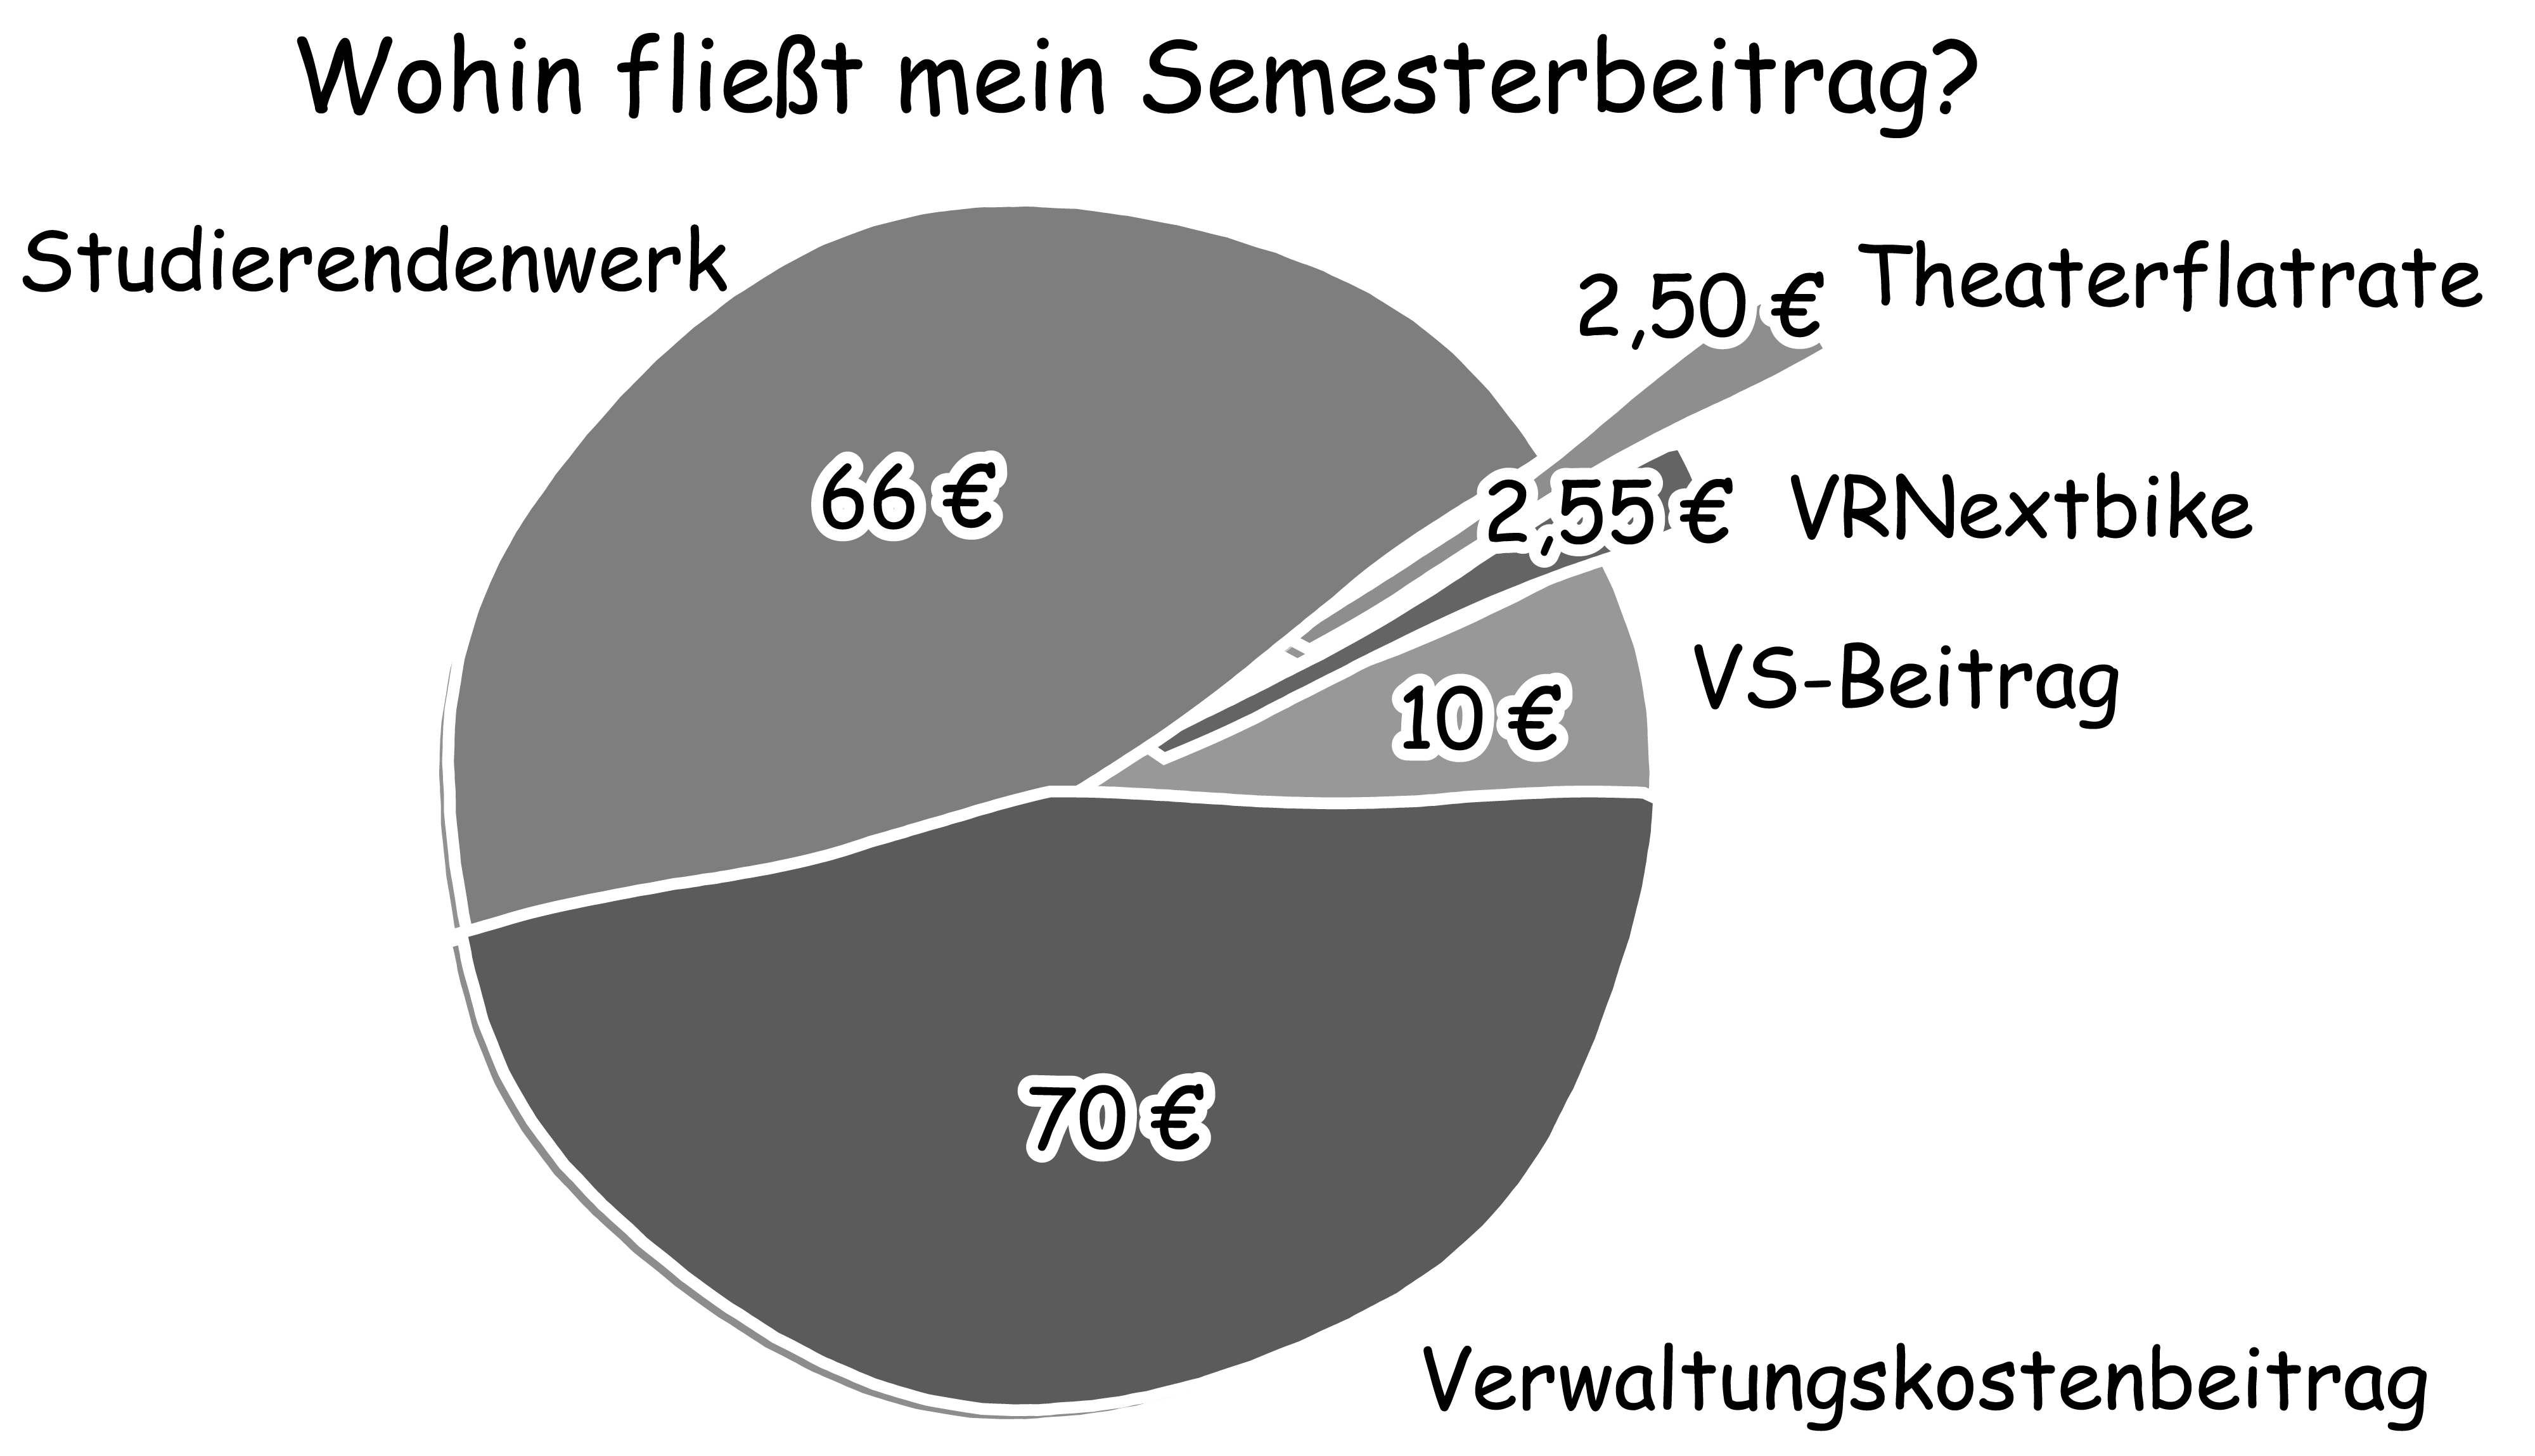
\includegraphics[width=\textwidth]{semesterbeitrag_grayscale.png}
    }{
        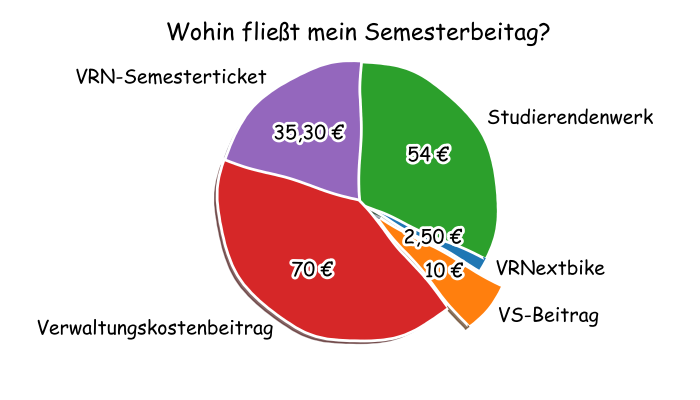
\includegraphics[width=\textwidth]{semesterbeitrag.png}
    }
\end{figure*}

\subsection{Verfasste Studierendenschaft (VS)}
Seit dem Wintersemester 2013/14 sind in Baden-Württemberg Verfasste Studierendenschaften wieder erlaubt.
Zuvor waren diese 1977 verboten worden, um Studentinnen vor politischen Dummheiten zu bewahren.
Bei der Wiedereinführung der VS wurde in einer Urabstimmung die organisatorische Struktur festgelegt:
An der Universität Heidelberg gibt es als legislatives Gremium den Studierendenrat (StuRa) und als exekutives Organ die Referatekonferenz (RefKonf), welche von den Vorsitzenden der Verfassten Studierendenschaft geleitet wird.

Im Studierendenrat kommen Vertreterinnen aus fast allen 51 Studienfachschaften zusammen.
Darüber hinaus können bis zu 50\% der Plätze durch gewählte Mitglieder von Hochschulgruppen besetzt werden, jedoch hängt die Anzahl von der Wahlbeteiligung ab, welche leider nicht sehr hoch ist.
Der StuRa tagt in der Regel zweiwöchentlich in öffentlichen Sitzungen, wo jede Studentin Antrags- und Rederecht besitzt.
Dort wird unter anderem über eingereichte Finanzanträge entschieden, denn über den Semesterbeitrag zahlen alle Studentinnen einen Beitrag von \EUR{\vsbeitrag} an die VS, wovon ein Teil an zentraler Stelle vergeben und der Rest an die Fachschaften aufgeteilt wird.
Außerdem wird auch hier aus Gremien berichtet, Kandidatinnen in Gremien gewählt, Satzungen oder Ordnungen beschlossen, und vor allem über alle allgemeinen Belange des studentischen Lebens diskutiert.

In der Referatekonferenz, welche auch zweiwöchentlich versetzt tagt, treffen sich die Referentinnen.
Diese werden vom StuRa für ein Jahr gewählt und befassen sich mit einem bestimmten Bereich (Justiz"=, Ökologie"=, Öffentlichkeits"=, Finanz"=, Kultur"=, Verkehrsreferat, etc.).
Für spezifische Anliegen und Projekte sind die Referate die besten Ansprechpartner, zum Beispiel das Kulturreferat, wenn die Sperrzeiten in der Altstadt sich ändern sollen.

\subsection{Überregionale Strukturen}
Da es nicht nur Studentinnen in Heidelberg gibt, sondern in ganz Baden-Württemberg, Deutschland und auf der ganzen Welt, gibt es natürlich auch hierfür studentische Interessensvertretungen.
In Deutschland ist Bildung Ländersache, deshalb richten sich bei uns erstmal alles nach dem Landeshochschulgesetz (LHG) von Baden"=Württemberg.
Die Verfassten Studierendenschaften treffen sich regelmäßig zu sogenannten Landes"=Asten"=Konferenzen (LAK) und vernetzen sich dort, zum Beispiel, wenn es um das Thema Studiengebühren oder eine Novelle des LGH geht.

Aber auch die dezentral organisierten Fachschaften stehen in ständigem Austausch.
Auf den Bundesfachschaftentagungen (BuFaTas) -- Konferenz der Mathematikfachschaften (KoMa), Konferenz der Informatik"=Fachschaften (KIF) und Zusammenkunft aller Physik"=Fachschaften (ZaPF) -- treffen sich Studentinnen der jeweiligen Fächer aus dem gesamten deutschsprachigen Gebiet jedes Semester.
Neben hochschulpolitischen Diskussionen und resultierenden Resolutionen stehen vor allem der Austausch und die Vernetzung im Vordergrund.
